% Unofficial University of Cambridge Poster Template
% https://github.com/andiac/gemini-cam
% a fork of https://github.com/anishathalye/gemini
% also refer to https://github.com/k4rtik/uchicago-poster

\documentclass[final]{beamer}

% ====================
% Packages
% ====================

\usepackage[T1]{fontenc}
\usepackage{lmodern}
\usepackage[orientation=portrait,size=a1]{beamerposter}
\usetheme{gemini}
\usecolortheme{nott}
\usepackage{graphicx}
\usepackage{booktabs}
\usepackage{tikz}
\usepackage{pgfplots}
\pgfplotsset{compat=1.14}
\usepackage{anyfontsize}
\usepackage{kotex}
\usepackage{amsmath}
\usepackage{mathtools}
\usepackage{amssymb}
\usepackage[labelformat=empty]{caption}
\usepackage{subcaption}
\usepackage{algpseudocode}
\setbeamerfont{block title}{size=\Large}
\setbeamerfont{block body}{size=\Large}



\captionsetup[subfigure]{labelformat=empty}

% ====================
% Lengths
% ====================

% If you have N columns, choose \sepwidth and \colwidth such that
% (N+1)*\sepwidth + N*\colwidth = \paperwidth
\newlength{\sepwidth}
\newlength{\colwidth}
% \setlength{\sepwidth}{0.025\paperwidth}
% \setlength{\colwidth}{0.45\paperwidth}

% \newcommand{\separatorcolumn}{\begin{column}{\sepwidth}\end{column}}


% ====================
% Title
% ====================

%\title{Arc Indices of Theta-Curves and Handcuff Graphs}
\title{Arc Index of Theta-curves and Handcuff-graphs}


\author{Cho, Eunchan \inst{1} \and  Shin, Jeongwon \inst{1} \and  Seo, Boyeon \inst{1} \and  Choi, Minho \inst{1} \and Kim, Hun \inst{2} \and Jin, GyoTaek \inst{3}}

\institute[shortinst]{\inst{1} Korea Science Academy of KAIST \samelineand \inst{2} Supervisor, Korea Science Academy of KAIST \samelineand \inst{3} Supervisor, Department of Mathematical Sciences, Korea Advanced Institute of Science and Technology \samelineand}

% ====================
% Footer (optional)
% ====================

\footercontent{
  \begin{center}
    \begin{minipage}[c]{\linewidth}
      \centering
      \makebox[0.3\linewidth][r]{%
        
\includegraphics[height=2cm]{logos/image.png}
      }%
      \makebox[0.4\linewidth][c]{%
        
\includegraphics[height=2cm]{logos/kaist_logo.png}
      }%
      \makebox[0.3\linewidth][l]{%
        
\includegraphics[height=2cm]{logos/gwagibu_logo.png}
      }
    \end{minipage}

    \vspace{0.3cm}

    Korea Science Academy of KAIST \quad
    \href{http://www.ksa.hs.kr}{ksa.hs.kr} \quad
  \end{center}
}


% ====================
% Logo (optional)
% ====================

% use this to include logos on the left and/or right side of the header:
% \logoright{
\includegraphics[height=2.4cm]{logos/utfpr-logo.png}}
% \logoleft{\hspace{20ex}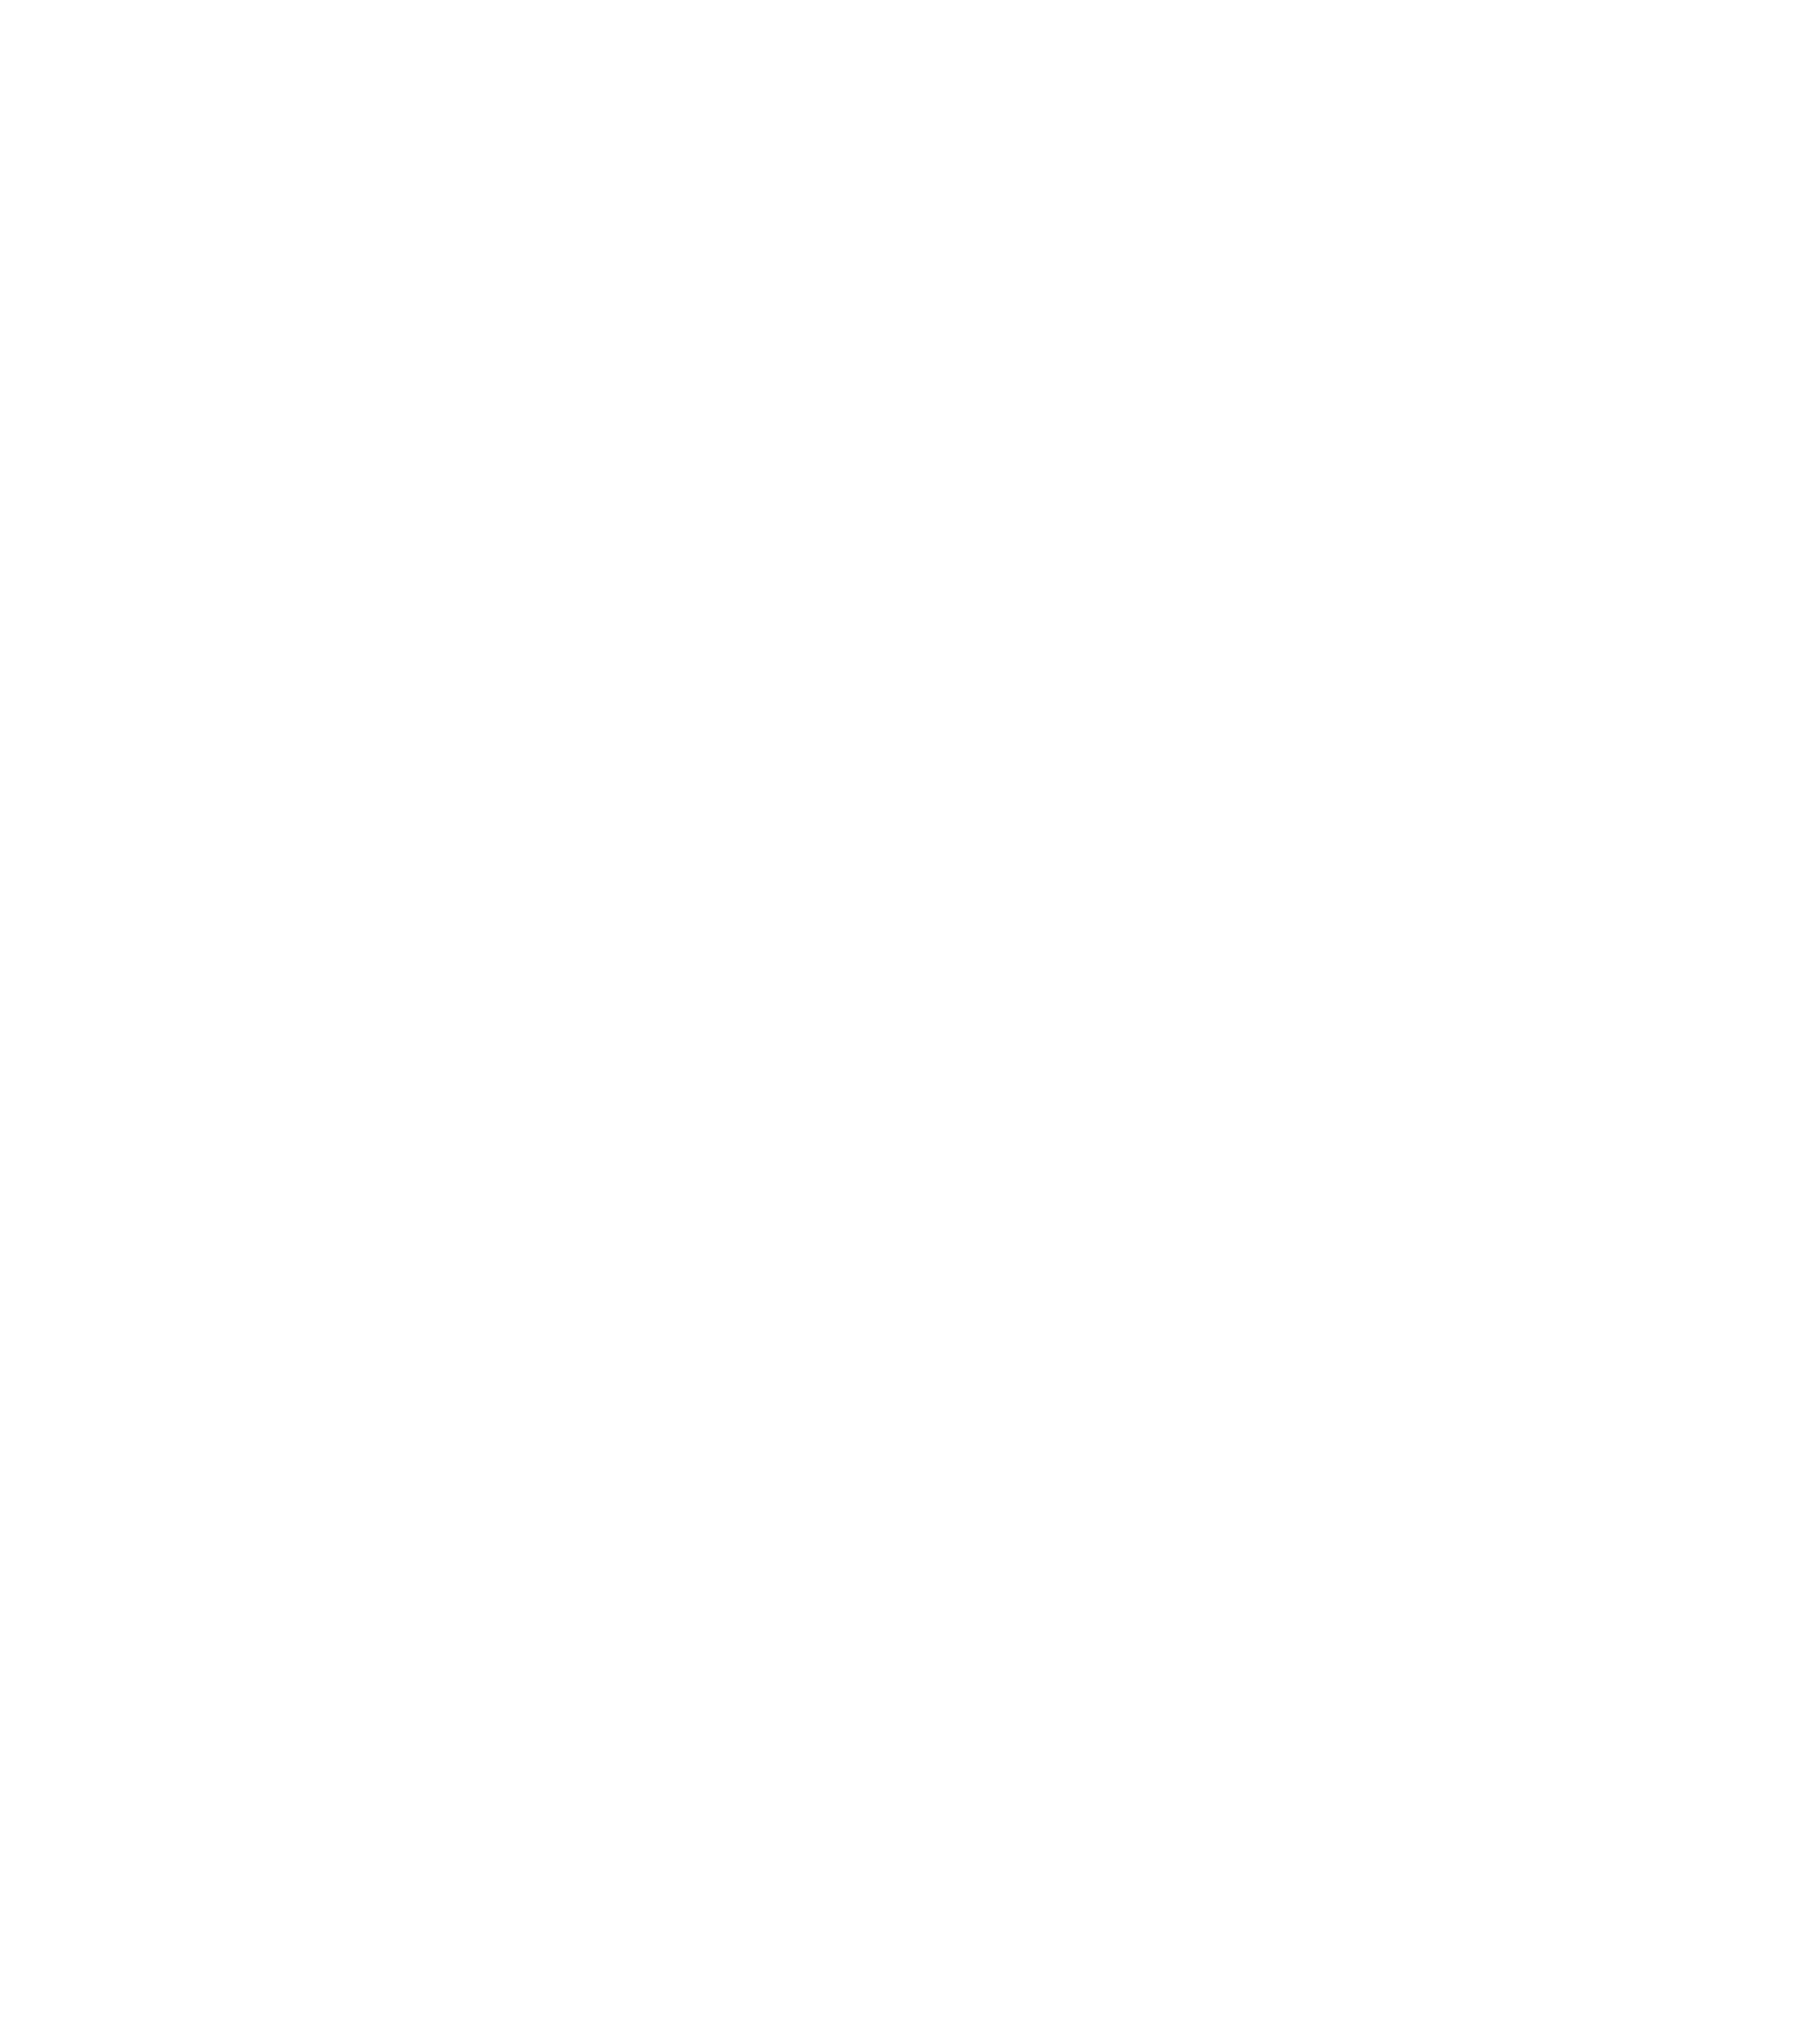
\includegraphics[height=3.5cm]{logos/ppgca-logo.png}}

% ====================
% Body
% ====================



\begin{document}

% Refer to https://github.com/k4rtik/uchicago-poster
% logo: https://www.cam.ac.uk/brand-resources/about-the-logo/logo-downloads
% \addtobeamertemplate{headline}{}
% {
%     \begin{tikzpicture}[remember picture,overlay]
%       \node [anchor=north west, inner sep=3cm] at ([xshift=-2.4cm,yshift=1.75cm]current page.north west)
%       {\includegraphics[height=7cm]{logos/unott-logo.eps}}; 
%     \end{tikzpicture}
% }

\begin{frame}[t]
% \begin{columns}[t]
% \separatorcolumn

% \begin{column}{\colwidth}
\begin{columns}[t]
  \column{0.33\textwidth}
  \begin{block}{Definitions}
    %\textbf{Knot} is an embedding of a circle in 3-dimensional Euclidean space.
    %In \textbf{Knot Theory}, people classify each knot using their \textbf{Knot Invariant}. \\
    \begin{itemize}
      \item \textbf{Theta-curve} : A graph embedded in $S^3$, consisting of two vertices and three edges, where each edge connects the two vertices.
      %In the projection of the theta-curve, the section where theta-curve meets itself is named \textbf{crossing}.
      %If the one theta-curve and other theta-curve's continuous transform of the graph is same, these curves are \textbf{equivalent}.
      \item \textbf{Handcuff graph} : A graph embedded in $S^3$, consisting of two vertices and three edges, where one edge connects the two vertices, and each of the other two edges forms a loop at one of the vertices.
      \item \textbf{Generalized Reidemeister move} : Five local moves on a spatial graph that does not alter the isotopy class of the spatial graph in $\mathbb{R}^3$.
    \end{itemize}
    \begin{figure}[h]
        \centering
        \begin{tabular}{ccc}
          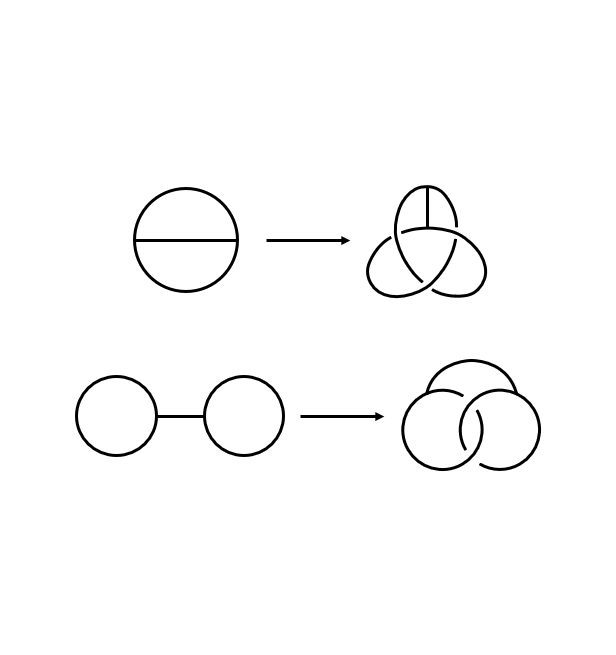
\includegraphics[width=0.43\textwidth]{figure/spatial_deformation.png} &
          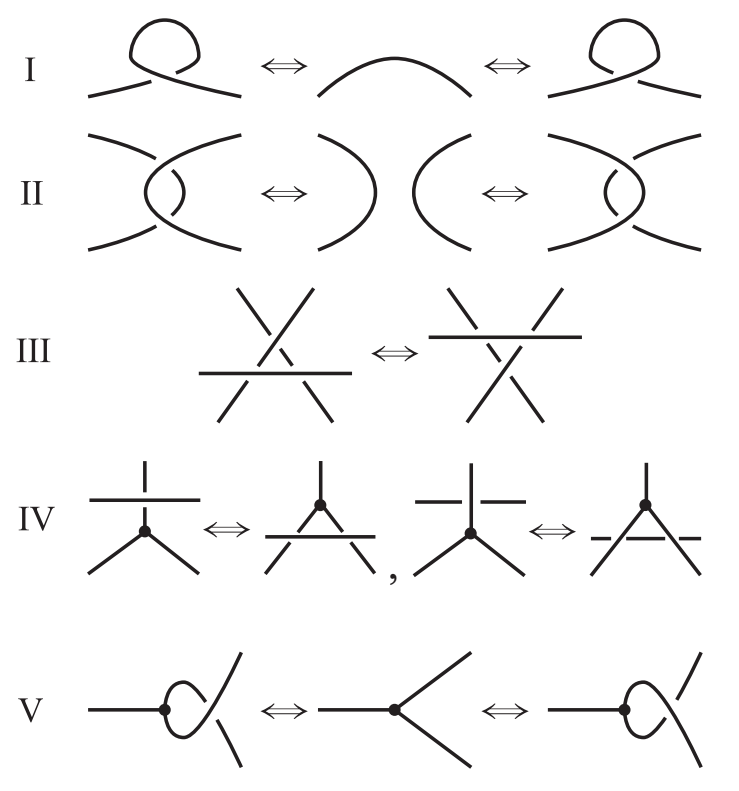
\includegraphics[width=0.43\textwidth]{figure/reidemeister.png} \\
        \end{tabular}
        \caption{$\theta$-curve, handcuff graph and generalized Reidemeister move}
    \end{figure}
  \end{block}

  \begin{block}{Diagrams}
    %\caption{An algorithm with caption}\label{alg:cap}
    \begin{itemize} 
      \item \textbf{Grid diagram}: A handcuff graph or $\theta$-curve diagram of vertical strands and one less number of horizontal strands with the properties that at every crossing the vertical strand crosses over the horizontal strand and no two horizontal segments are co-linear and no two vertical segments are co-linear.
      \item \textbf{Cromwell matrix}: An $n\times n$ binary matrix each of whose rows and columns has exactly two $1$s. For $\theta$-curve and handcuff graph, its cromwell matrix is an $n\times(n{+}1)$ binary matrix that exactly two rows (called \textit{Three-rows}) has exactly three $1$s and rest of the rows and each columns has exactly two $1$s.
      \item \textbf{Arc presentation}: There is an open-book decomposition of $\mathbb{R}^3$ which has open half-planes as pages and the standard z-axis as the binding axis. Every spatial graph $G$ can be embedded in an open-book decomposition with finitely many pages so that it meets each page in exactly one simple arc with two different end-points on the binding axis.
      \item \textbf{Arc index} : The minimal number of pages among all possible arc presentations of K.
    \end{itemize}

    \begin{figure}[h]
      \centering
      \begin{tabular}{cc}
        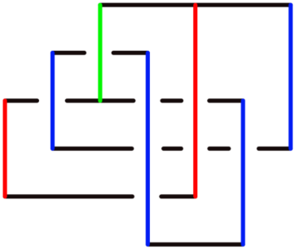
\includegraphics[width=0.4\textwidth]{figure/grid.png} &
        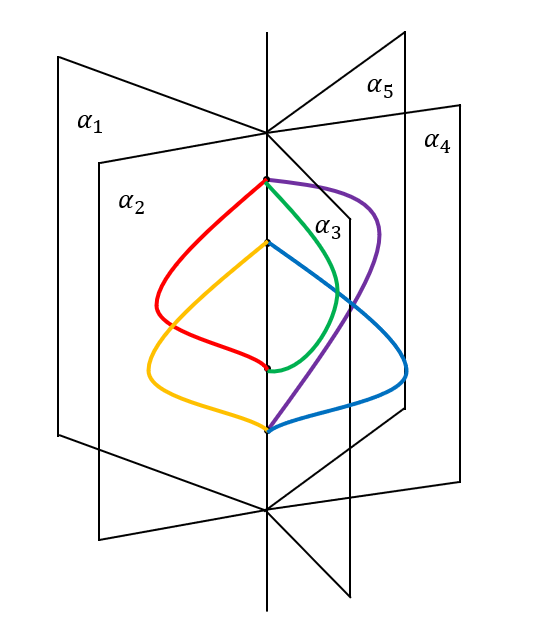
\includegraphics[width=0.4\textwidth]{figure/handcuff_openbook.png} \\
      \end{tabular}        
      \caption{Grid diagram of $\theta$-curve $3_1$ and arc presentation of handcuff graph $2_1$}
    \end{figure}
  \end{block}
    


  \column{0.33\textwidth}
  \begin{block}{Classifying $\theta$-Curves and Handcuff Graphs}
  \textbf{H-deletion matrix} : An $(n{-}1)\times(n{-}1)$ matrix after removing any \textit{Three-row} and the columns of its leftmost and rightmost $1$s from a cromwell matrix of a $\theta$-curve or handcuff graph. 

  \vspace{0.33em}
  
  $\mathbf{Theorem\ 1.}$ Let $G$ be a $\theta$-curve or handcuff graph, and the $H$ be a H-deletion matrix. Then,
  $G$ is a $\theta$-curve if and only if $\det{H} = \pm 1$, and $G$ is a handcuff graph if and only if $\det{H} = 0 \text{ or } \pm2$.
  \begin{figure}[h]
    \centering
    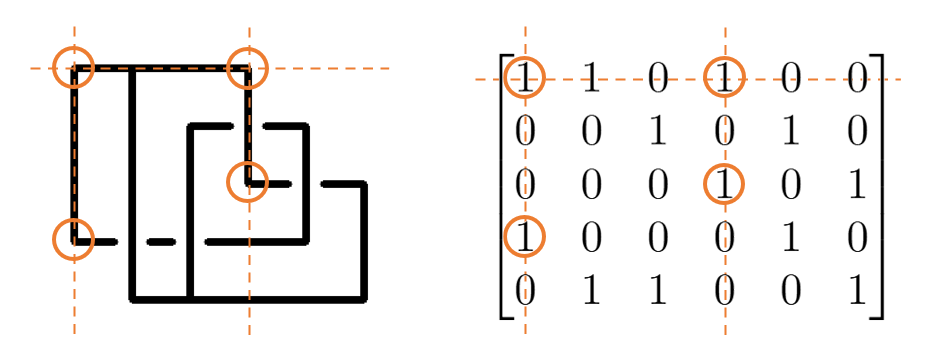
\includegraphics[width=0.8\textwidth]{figure/Hdeletion.png}
    \caption{H-deletion of $\theta$-curve graph $3_1$}
  \end{figure}
  \end{block}

  
  \begin{block}{Stacked Tangle Representation}
    \begin{itemize}
      \item \textbf{Non-simple disk} : A disk which contains one vertex and three line segments which joins the vertex and boundary point. 
      \item \textbf{Simple disk} : A disk which contains simple arc which joins two points on the boundary.
      \item \textbf{Stacked tangle} : Stacked disks each with the frame as boundary. Only two disks of the stacked tangle are non-simple disks(one is at the top), and others are simple disks. \\
      %\item \textbf{Arcs} : Segments properly embedded in each disk, with endpoints on the boundary
      \item \textbf{Caps} : Simple arc in outside of stacked tangle joining end points of arcs or line segments. \\
    \end{itemize}
    \begin{figure}
      \centering
      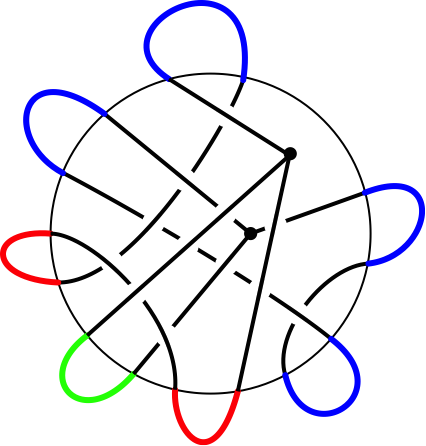
\includegraphics[width=0.4\textwidth]{figure/stacked_theta.png}
      \caption{Stacked tangle of handcuff graph}
    \end{figure}
    \begin{itemize}
      \item An arc in simple disk and arc in other simple disk or tree in non-simple disk intersect at most one point, and any two caps have no intersection when viewed from above.
    \end{itemize}
    \begin{figure}
      \centering
      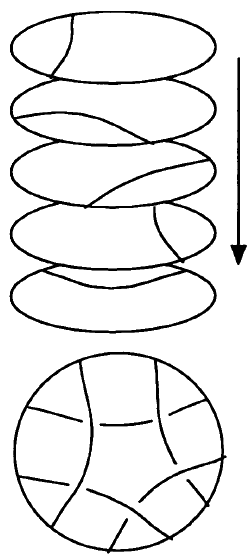
\includegraphics[width=0.7\textwidth]{figure/stacked_tangle.png}
      \caption{Stacked tangle and simple closure of handcuff graph $2_1$}
    \end{figure}
    \begin{itemize}
      \item \textbf{Reduced simple closure of a stacked tangle} : A simple closure of a stacked tangle without any nested caps. Any two arcs (including line segment) joining by caps have no intersection when viewed from above.
    %\item \textbf{Simple closure}: The planar projection of the stacked tangle without any nested caps
    \end{itemize}
  \end{block}

  
  \column{0.33\textwidth}
  \begin{block}{Bounds of Arc Index}
  $\mathbf{Theorem\ 2.}$ $[$3$]$ For any spatial graph $G$, 
  \begin{equation*}
    \alpha(H) \leq c(H) + e + b
  \end{equation*}
  where $\alpha (G)$, $c(G)$ are each arc index, crossing number of $G$, $e$ is the number of edges, and $b$ is the number of bouquet cut-components.
  
  $\mathbf{Corollary\ 1.}$ For non-trivial handcuff graph $H$,
  \begin{equation*}
    \alpha(H) \leq c(H) + 3
  \end{equation*}

 % $\mathbf{Theorem.}$ If H is handcuff, then 
 % \begin{equation*}
  %  \alpha(H) \geq \frac{1+\sqrt{f(\alpha(H)) + 36c(H)}}{3}
 % \end{equation*}
  %where
 % \begin{equation*}
  %  f(x) =
   % \begin{cases}
  %  73 & (x \equiv 0 \pmod{6}) \\
 %   4 & (x \equiv 1 \pmod{6}) \\
 %   25 & (x \equiv 2 \pmod{6}) \\
 %   -8 & (x \equiv 3 \pmod{6}) \\
 %   49 & (x \equiv 4 \pmod{6}) \\
  %  -20 & (x \equiv 5 \pmod{6})
 %   \end{cases}
 % \end{equation*}

  %$\mathbf{Theorem.}$ If $L$ is non-split alternating link, then 
  %\begin{equation*}
   % \alpha(L) = c(L)+2
  %\end{equation*}


  $\mathbf{Theorem\ 3.}$ Let $H$ be a handcuff graph and $L$ is link that connecting edge is deleted from $H$. If $L$ is non-split alternating, then 
  \begin{equation*}
    \alpha(H) \geq c(L) + 3
  \end{equation*}

    $\mathbf{Definition\ 1.}$ $[$5$]$ For a graph $G$, let
    \[ h(G)(x, y) = \sum_{F \subset E} (-x)^{-|F|} x^{\mu(G-F)} y^{\beta(G-F)} \]
    where $\mu(G)$, $\beta(G)$, and $E$ are the number of connected components, the first Betti number, and the edge set of $G$ each. Therefore, the \\
    \textbf{Yamada polynomial} of $G$, $R(G)$, is defined by
    \[ R(G)(x) = h(G)(-1, -x-2-x^{-1}). \]

    %\vspace{1em}

    %$\mathbf{Theorem.}$ $[$5$]$ For a spatial graph $G$, $(-x)^n R(G)$ is an ambient isotopy invariant for some integer $n$.

    %\vspace{1em}
    
    $\mathbf{Theorem\ 4.}$ $[$1$]$ Let $S_T$ be a simple closure of stacked tangle of a theta-curve or handcuff graph, and let $n$ be the number of crossings in $S_T$. Then,
     \[ \mathrm{spr}(R(S_T)) \leq 2n+2 \]
     where $\mathrm{spr}(f)$ denotes the difference between the maximal and minimal degrees of $f$. \\

    %\vspace{1em}

    $\mathbf{Corollary\ 2.}$ Let $G$ be a theta-curve or handcuff graph. Then, the arc index of $G$ is bounded by
      \[ \alpha(G) \geq \frac{5 + \sqrt{4 \mathrm{spr}(R(G)) - 15}}{2}. \]
  \end{block}

  \begin{block}{Further Studies}
    \begin{itemize}
      \item Fixing every arc index of handcuff graph and $\theta$-curve graph under $7$ crossings.
      \item Applying bounds of spatial graphs to knots.
    \end{itemize}
  \end{block}

  \begin{block}{Refernces}
    \begin{enumerate}
      \item Yoonsang Lee. (2023). \textit{A Study on Arc Index of Theta-Curves}. Korea Science Academy of KAIST
      \item Lee, H. J., Hong, K., Lee, H., \& Oh, S. (2014). Mosaic number of knots. \textit{Journal of Knot Theory and Its Ramifications, 23}(13), 1450069.
      \item Lee, M. J., No, S., \& Oh, S. (2018). Arc index of spatial graphs. \textit{Journal of Graph Theory, 90}(3), 406–415.
      \item Moriuchi, H. (2019). A table of $\theta$-curves and handcuff graphs with up to seven crossings. \textit{Advanced Studies in Pure Mathematics}, 281–290.
      \item Yamada, S. (1989). An invariant of spatial graphs. \textit{Journal of Graph Theory, 13}(5), 537–551.
      
    \end{enumerate}
  \end{block}

\end{columns}

\end{frame}

\end{document}